% Created 2016-08-17 Wed 14:38
\documentclass[tikz]{standalone}

\usepackage[utf8]{inputenc}
\usepackage[T1]{fontenc}

\usepackage{circledsteps}

\RequirePackage{xcolor}

%% HPI color definitions according to the design manual
% These do not exactly match the RGB values used in the Powerpoint slide master due to unknown reasons
\definecolor{hpiyellow}{RGB}{246,168,0}
\definecolor{hpiorange}{RGB}{221,97,8}
\definecolor{hpired}{RGB}{177,6,58}
\definecolor{hpigray}{RGB}{90,96,101}
\definecolor{hpiblue}{RGB}{0,122,158}


\renewcommand{\sfdefault}{neosans}
% Different font weights for neosans
\newcommand{\textl}[1]{{\fontseries{l}\selectfont #1}} % light
\newcommand{\textm}[1]{{\fontseries{m}\selectfont #1}} % medium, same as default weight
\newcommand{\textsb}[1]{{\fontseries{sb}\selectfont #1}} % semibold
\newcommand{\textmb}[1]{{\fontseries{mb}\selectfont #1}} % bold, same as \textbf
\newcommand{\texteb}[1]{{\fontseries{eb}\selectfont #1}} % extra bold
\newcommand{\textub}[1]{{\fontseries{ub}\selectfont #1}} % ultra bold

\tikzset{every picture/.style={/utils/exec={\sffamily}}}
\tikzset{flipflop RSflanke/.style={
  flipflop,
  flipflop def={t1=S, t2=C, c2=1, t3=R, t6=Q, t4={\ctikztextnot{Q}}}
}}


\tikzset{
  mechanicalSwitch/.pic={
    \coordinate (-inUp) at (135:2); 
    \coordinate (-inDown) at (235:2);
    \coordinate (-out) at (2,0);
    \coordinate (-center) at (0,0);
    
    \draw (0,0) circle [radius = 2cm];
    \draw [fill=gray!20] (0,0) circle [radius = 0.2cm];

    \draw (0, 0) -- (2, 0);
    \draw (135:.8) -- (135:2); 
    \draw (225:.8) -- (225:2); 

    \draw [fill=gray!20] (2, 0) circle [radius=0.05cm]; 
    \draw [fill=gray!20] (135:2) circle [radius=0.05cm]; 
    \draw [fill=gray!20] (225:2) circle [radius=0.05cm]; 

    
    \draw [thick] (0,0) -- (175:1.5); 

    \draw [dashed, <->, domain=135:225] plot ({cos(\x)}, {sin(\x)}); 
  },
  mechanicalSwitchClosed/.pic={
    \coordinate (-inUp) at (135:2); 
    \coordinate (-inDown) at (255:2);
    \coordinate (-out) at (2,0);
    \coordinate (-center) at (0,0);
    \draw (0,0) circle [radius = 2cm];
    \draw [fill=gray!20] (0,0) circle [radius = 0.2cm];

    \draw (0, 0) -- (2, 0);
    \draw (135:.8) -- (135:2); 
    \draw (225:.8) -- (225:2); 

    \draw [fill=gray!20] (2, 0) circle [radius=0.05cm]; 
    \draw [fill=gray!20] (135:2) circle [radius=0.05cm]; 
    \draw [fill=gray!20] (225:2) circle [radius=0.05cm]; 

    
    \draw [thick] (0,0) -- (135:2); 

    \draw [dashed, <->, domain=135:225] plot ({cos(\x)}, {sin(\x)}); 
  }
}


\usetikzlibrary{calc}
\usetikzlibrary{positioning}


\usepackage{ifthen}


\usetikzlibrary{automata}
\usetikzlibrary{arrows}       %                 ...customizing arrows
\usetikzlibrary{decorations.pathreplacing,decorations.pathmorphing}       %                 ...customizing arrows


\tikzset{node distance=5cm, % Minimum distance between two nodes. Change if necessary.
  every node/.style={           align=center,
},
         every state/.style={ % Sets the properties for each state
           semithick,
           fill=gray!10},
         initial text={},     % No label on start arrow
         double distance=2pt, % Adjust appearance of accept states
         every edge/.style={  % Sets the properties for each transition
           draw, ->, 
           % ->,>=stealth’,     % Makes edges directed with bold arrowheads
           auto,
           semithick}}

       
\begin{document}

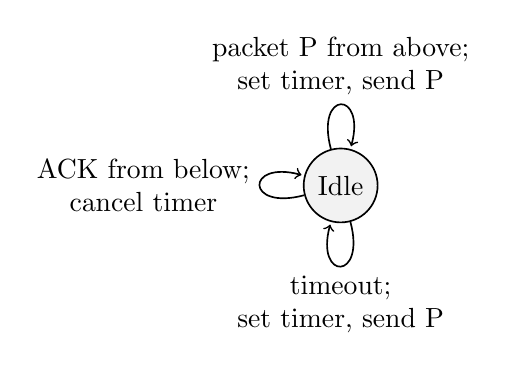
\begin{tikzpicture}
  \label{page:arq:simple_sender}

  \node [state] (qidle) {Idle};

  \draw (qidle) edge [loop above] node[above] {
    packet P from above;\\
    set timer, send P
  } (qidle); 

  \draw (qidle) edge [loop left] node[left] {
    ACK from below;\\
    cancel timer
  } (qidle); 

  \draw (qidle) edge [loop below] node[below] {
    timeout;\\
    set timer, send P
  } (qidle);   
\end{tikzpicture}

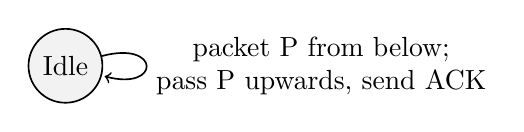
\begin{tikzpicture}
  \label{page:arq:simple_receiver}

  \node [state] (qidle) {Idle};
  
  \draw (qidle) edge [loop right] node[right] {
    packet P from below; \\
    pass P upwards, send ACK 
  } (qidle); 

\end{tikzpicture}


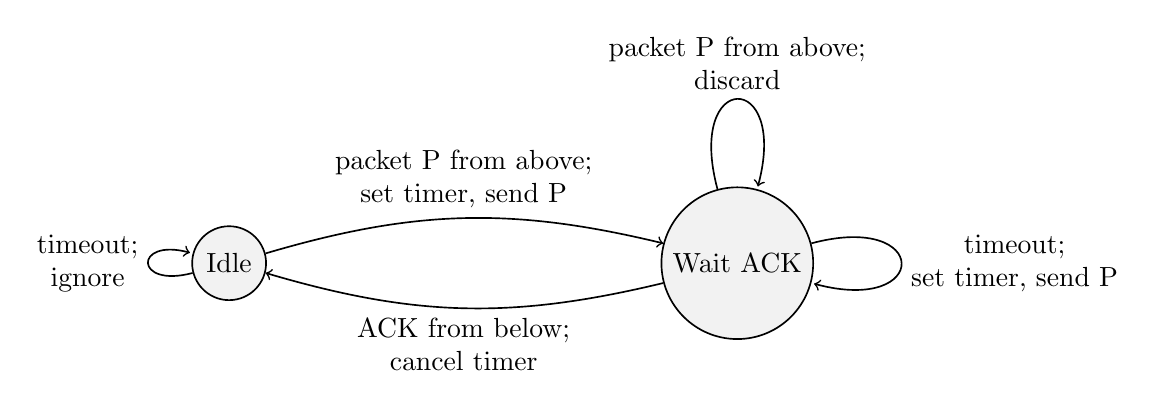
\begin{tikzpicture}
  \label{page:arq:sender_process}

  \node [state] (qidle) {Idle};
  \node [state, right=of qidle] (qwait) {Wait ACK}; 

  \draw (qidle) edge [bend left=15] node[above] {
    packet P from above;\\
    set timer, send P
  } (qwait); 

  \draw (qwait) edge [loop above] node[above] {
    packet P from above;\\
    discard
  } (qwait); 

  \draw (qwait) edge [loop right] node[right] {
    timeout;\\
    set timer, send P
  } (qwait);   
  
  \draw (qwait) edge [bend left=15] node[below] {
    ACK from below;\\
    cancel timer
  } (qidle); 

  \draw (qidle) edge [loop left] node[left] {
    timeout;\\
    ignore
  } (qidle);   
\end{tikzpicture}


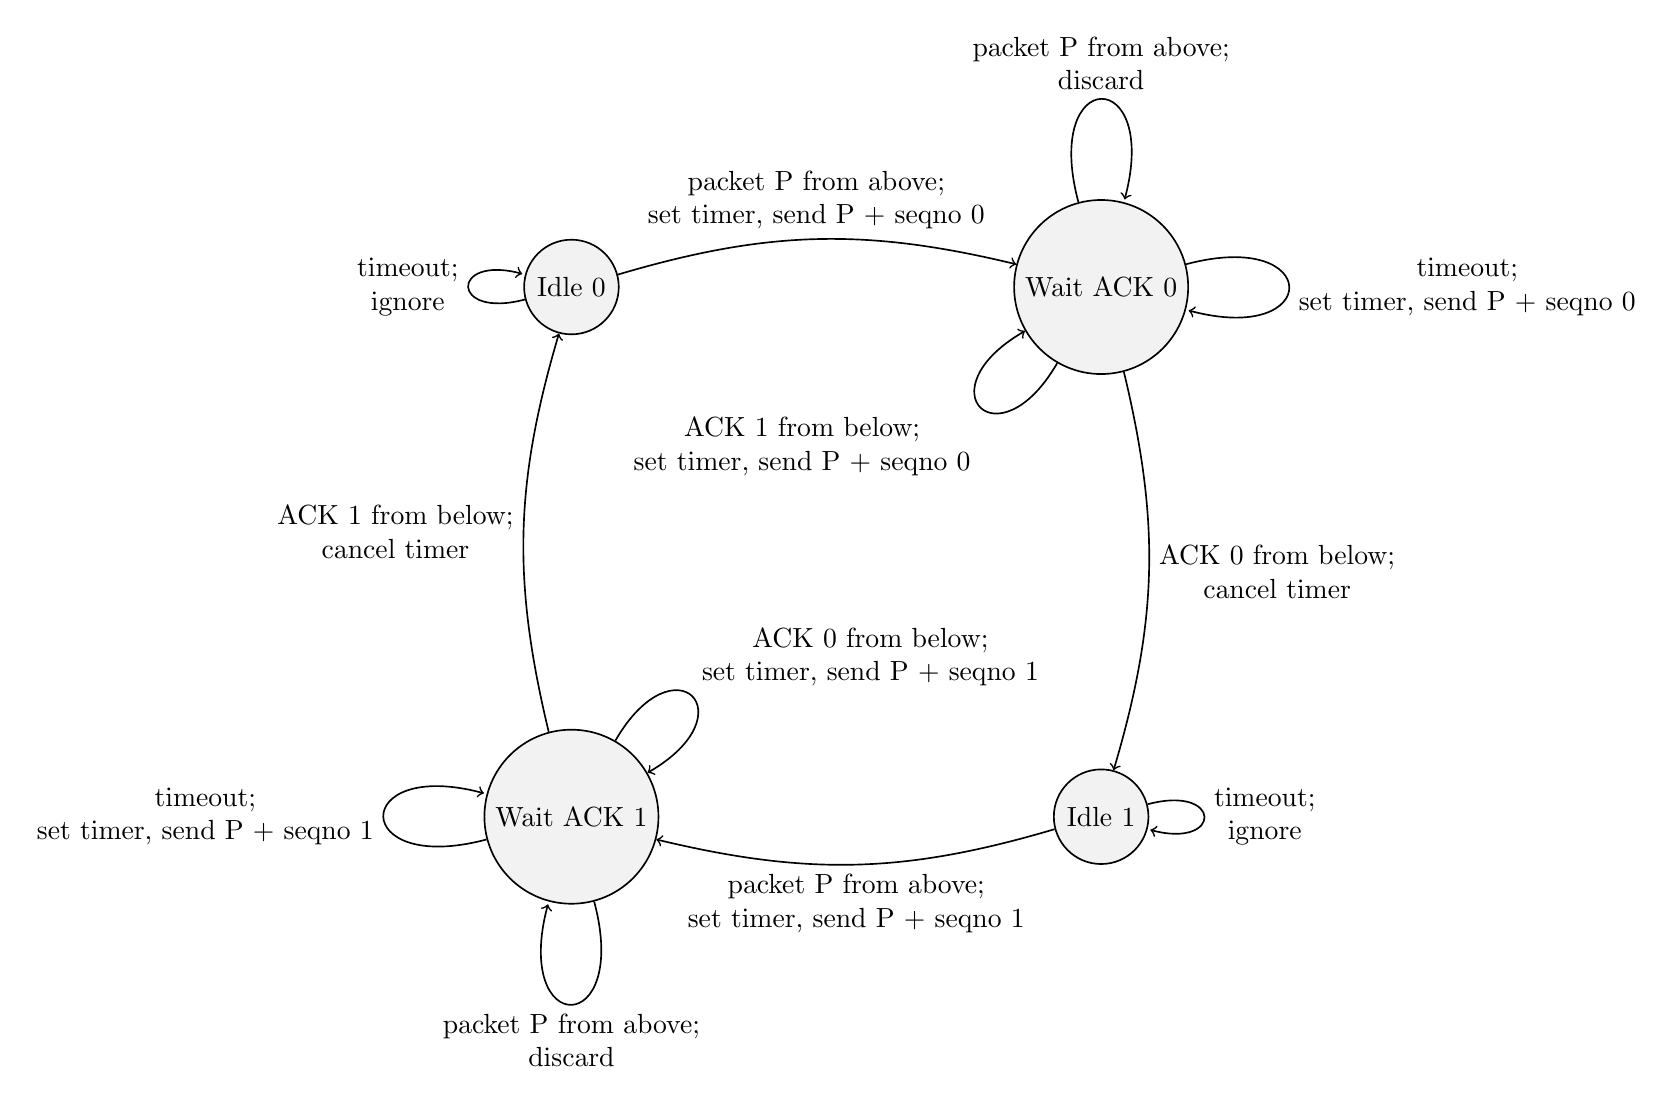
\begin{tikzpicture}
  \label{page:arq:sender_alternating_bit}

  \node [state] (qidle0) {Idle 0};
  \node [state, right=of qidle0] (qwait0) {Wait ACK 0}; 
  \node [state, below=of qwait0] (qidle1) {Idle 1};
  \node [state, below=of qidle0] (qwait1) {Wait ACK 1}; 

  
  \draw (qidle0) edge [bend left=15] node[above] {
    packet P from above;\\
    set timer, send P + seqno 0
  } (qwait0); 

  \draw (qidle1) edge [bend left=15] node[below] {
    packet P from above;\\
    set timer, send P + seqno 1
  } (qwait1); 
  
  \draw (qwait0) edge [loop above] node[above] {
    packet P from above;\\
    discard
  } (qwait0); 

  \draw (qwait1) edge [loop below] node[below] {
    packet P from above;\\
    discard
  } (qwait1); 
  
  \draw (qwait0) edge [loop right] node[right] {
    timeout;\\
    set timer, send P + seqno 0
  } (qwait0);   

  \draw (qwait1) edge [loop left] node[left] {
    timeout;\\
    set timer, send P + seqno 1
  } (qwait1);   
  
  \draw (qwait0) edge [bend left=15] node[right] {
    ACK 0 from below;\\
    cancel timer
  } (qidle1); 

  \draw (qwait1) edge [bend left=15] node[left] {
    ACK 1 from below;\\
    cancel timer
  } (qidle0); 
  
  \draw (qidle0) edge [loop left] node[left] {
    timeout;\\
    ignore
  } (qidle0);   

  \draw (qidle1) edge [loop right] node[right] {
    timeout;\\
    ignore
  } (qidle1);

  % and wrong ACKs:
  \draw (qwait0) edge [loop, out=240, in=210, min distance=15mm] node[below left] {
    ACK 1 from below;\\
    set timer, send P + seqno 0
  } (qwait0); 

  \draw (qwait1) edge [loop, out=60, in=30, min distance=15mm] node[above right] {
    ACK 0 from below;\\
    set timer, send P + seqno 1
  } (qwait1); 
  
\end{tikzpicture}

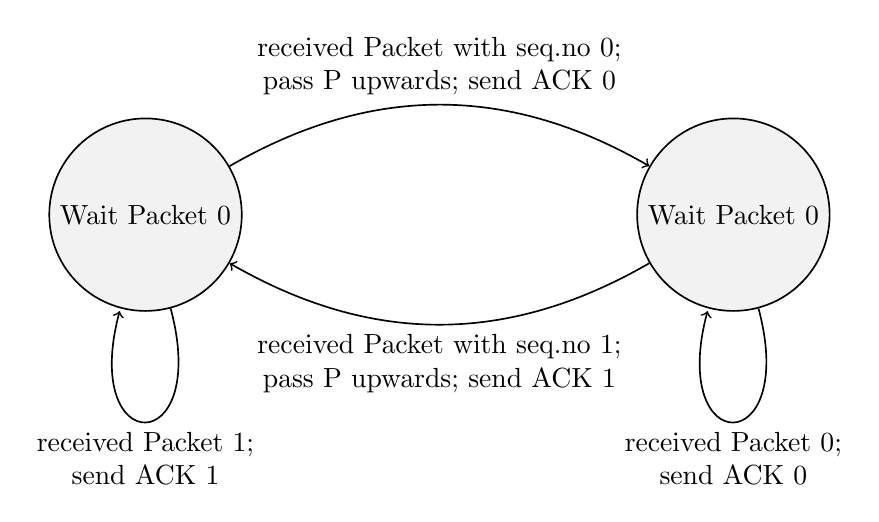
\begin{tikzpicture}
  \label{page:ll:receiver_alternating_bit}
  \node [state] (qwait0) {Wait Packet 0}; 
  \node [state, right=of qwait0] (qwait1) {Wait Packet 0};

  \draw (qwait0) edge [loop below] node [below] {
    received Packet 1; \\
    send ACK 1
    } (qwait0); 


  \draw (qwait1) edge [loop below] node [below] {
    received Packet 0; \\
    send ACK 0
  } (qwait1);

  \draw (qwait0) edge [bend left] node[above] {
    received Packet with seq.no 0; \\
    pass P upwards; send ACK 0
  } (qwait1); 

  \draw (qwait1) edge [bend left] node[below] {
    received Packet with seq.no 1; \\
    pass P upwards; send ACK 1
  } (qwait0); 
  
  

\end{tikzpicture}



\end{document}